\documentclass[11pt]{article}
\usepackage[margin=0.7in]{geometry}
\usepackage{booktabs,amsmath,amssymb,graphicx,subcaption}
\newcommand{\sym}[1]{\ifmmode^{#1}\else\(^{#1}\)\fi}
\setlength{\parindent}{0pt}
\begin{document}
\begin{center}\large\textbf{Table 5 extension: CEIV and CEIC}\end{center}
\begin{center}\small
\begin{tabular}{lcccc}\toprule
&\multicolumn{1}{c}{(1)}&\multicolumn{1}{c}{(2)}&\multicolumn{1}{c}{(3)}&\multicolumn{1}{c}{(4)}\\
\midrule
\multicolumn{5}{l}{\textit{Panel A: Group CCEI -- OLS}}\\
$\text{CCEI}_{\text{max},gt}$&    0.127        &    0.121        &    0.131        &    0.077        \\
                &  (0.098)        &  (0.095)        &  (0.095)        &  (0.116)        \\
$\text{CCEI}_{\text{min},gt}$&    0.234\sym{**}&    0.228\sym{**}&    0.235\sym{**}&    0.162\sym{**}\\
                &  (0.045)        &  (0.044)        &  (0.045)        &  (0.045)        \\
\midrule
N               &     1304        &     1304        &     1304        &     1304        \\
R-squared       &    0.166        &    0.186        &    0.197        &    0.637        \\

\midrule
\multicolumn{5}{l}{\textit{Panel B: Group CEI -- OLS}}\\
$\text{CCEI}_{\text{max},gt}$&    0.252\sym{**}&    0.257\sym{**}&    0.250\sym{**}&    0.221\sym{*} \\
                &  (0.093)        &  (0.090)        &  (0.089)        &  (0.104)        \\
$\text{CCEI}_{\text{min},gt}$&    0.007        &    0.008        &    0.012        &   -0.054        \\
                &  (0.023)        &  (0.023)        &  (0.023)        &  (0.041)        \\
\midrule
N               &     1304        &     1304        &     1304        &     1304        \\
R-squared       &    0.083        &    0.101        &    0.103        &    0.568        \\
\midrule
\multicolumn{5}{l}{\textit{Panel C: Group CEIV -- OLS}}\\
$\text{CCEI}_{\text{max},gt}$&    0.171\sym{+} &    0.177\sym{+} &    0.176\sym{+} &    0.192\sym{+} \\
                &  (0.100)        &  (0.095)        &  (0.094)        &  (0.111)        \\
$\text{CCEI}_{\text{min},gt}$&    0.084\sym{*} &    0.081\sym{*} &    0.086\sym{*} &    0.001        \\
                &  (0.035)        &  (0.034)        &  (0.035)        &  (0.045)        \\
\midrule
N               &     1304        &     1304        &     1304        &     1304        \\
R-squared       &    0.095        &    0.111        &    0.115        &    0.586        \\

\midrule
\multicolumn{5}{l}{\textit{Panel D: Group CEIC -- OLS}}\\
$\text{CCEI}_{\text{max},gt}$&    0.227\sym{*} &    0.226\sym{*} &    0.241\sym{*} &    0.171        \\
                &  (0.108)        &  (0.103)        &  (0.100)        &  (0.126)        \\
$\text{CCEI}_{\text{min},gt}$&    0.202\sym{**}&    0.197\sym{**}&    0.204\sym{**}&    0.100\sym{+} \\
                &  (0.046)        &  (0.045)        &  (0.045)        &  (0.050)        \\
\midrule
N               &     1304        &     1304        &     1304        &     1304        \\
R-squared       &    0.149        &    0.169        &    0.181        &    0.633        \\

\midrule Fixed effects & Class & Class & Class & Pair \\ Student and friendship controls & & \checkmark & \checkmark & \checkmark \\ Corner/midpoint share controls & & & \checkmark & \checkmark \\ \bottomrule

\end{tabular}\end{center}
\small
\textit{Notes:} Panels A and B reproduce the current draft without re-estimation;
Panels C and D use the new workbook indices. The specifications are identical to
Table 5: class fixed effects in columns (1)--(3), pair fixed effects in column (4),
student and friendship controls in (2)--(4), and choice-pattern controls in (3)--(4).
Risk-aversion controls are excluded. Standard errors are clustered by 64 classes.
All models use 1,304 pair-waves from 652 pairs.
+, *, and ** denote significance at the 10\%, 5\%, and 1\% levels.

\medskip
One supplied CEIC midpoint (0.83875) has an unresolved interval [0.836, 0.8415].
The supplied midpoint is retained. The draft has not been edited.
\clearpage
\begin{center}\large\textbf{Table 5 extension: Fractional-response models}\end{center}
\begin{center}\small
\begin{tabular}{lcccc}\toprule
& (1) & (2) & (3) & (4) \\
\midrule
\multicolumn{5}{l}{\textit{Panel A: Group CCEI}}\\
$\text{CCEI}_{\text{max},gt}$&    0.077        &    0.077        &    0.094\sym{+} &    0.017        \\
                &  (0.054)        &  (0.050)        &  (0.051)        &  (0.078)        \\
$\text{CCEI}_{\text{min},gt}$&    0.176\sym{**}&    0.171\sym{**}&    0.184\sym{**}&    0.118\sym{**}\\
                &  (0.023)        &  (0.023)        &  (0.022)        &  (0.029)        \\
\midrule
N               &     1304        &     1304        &     1304        &     1304        \\


\midrule
\multicolumn{5}{l}{\textit{Panel B: Group CEI}}\\
$\text{CCEI}_{\text{max},gt}$&    0.176\sym{**}&    0.187\sym{**}&    0.182\sym{**}&    0.128\sym{+} \\
                &  (0.056)        &  (0.053)        &  (0.053)        &  (0.073)        \\
$\text{CCEI}_{\text{min},gt}$&    0.009        &    0.008        &    0.011        &   -0.051        \\
                &  (0.021)        &  (0.022)        &  (0.022)        &  (0.034)        \\
\midrule
N               &     1304        &     1304        &     1304        &     1304        \\


\midrule
\multicolumn{5}{l}{\textit{Panel C: Group CEIV}}\\
$\text{CCEI}_{\text{max},gt}$&    0.121\sym{+} &    0.133\sym{*} &    0.134\sym{*} &    0.108        \\
                &  (0.064)        &  (0.058)        &  (0.057)        &  (0.083)        \\
$\text{CCEI}_{\text{min},gt}$&    0.072\sym{**}&    0.067\sym{**}&    0.072\sym{**}&   -0.004        \\
                &  (0.026)        &  (0.026)        &  (0.026)        &  (0.034)        \\
\midrule
N               &     1304        &     1304        &     1304        &     1304        \\


\midrule
\multicolumn{5}{l}{\textit{Panel D: Group CEIC}}\\
$\text{CCEI}_{\text{max},gt}$&    0.156\sym{*} &    0.161\sym{*} &    0.184\sym{**}&    0.083        \\
                &  (0.071)        &  (0.065)        &  (0.063)        &  (0.091)        \\
$\text{CCEI}_{\text{min},gt}$&    0.167\sym{**}&    0.160\sym{**}&    0.171\sym{**}&    0.072\sym{+} \\
                &  (0.031)        &  (0.030)        &  (0.030)        &  (0.039)        \\
\midrule
N               &     1304        &     1304        &     1304        &     1304        \\
\midrule Link & Logit & Logit & Logit & Probit \\ Class fixed effects & \checkmark & \checkmark & \checkmark & \checkmark \\ Student and friendship controls & & \checkmark & \checkmark & \checkmark \\ Corner/midpoint share controls & & & \checkmark & \checkmark \\ Pair means and wave effect & & & & \checkmark \\ \bottomrule

\end{tabular}\end{center}
\small
\textit{Notes:} Average partial effects. Columns (1)--(3) use fractional logit with
class fixed effects. Column (4) follows the existing panel fractional probit
specification, adding pair means of the individual CCEIs and time-varying controls,
a wave effect, and class fixed effects. It does not use conditional logit or pair
fixed effects. Pair means are held fixed when computing the column (4) derivatives.
The control sets match the corresponding OLS columns; risk-aversion controls are
excluded throughout. Effects are per unit of individual CCEI; multiply by 0.1
for a 0.1 increase. Class-clustered standard errors are in parentheses.
All models use 1,304 pair-waves from 652 pairs in 64 classes.
+, *, and ** denote significance at the 10\%, 5\%, and 1\% levels.

\medskip
Panels A and B provide the existing CCEI and CEI specifications for comparison;
Panels C and D extend them to CEIV and CEIC. All four panels are estimated on the
validated analysis sample. The supplied CEIC midpoint and its numerical caveats
are retained as described on the preceding page and in the Figure 6 notes.
\clearpage
\begin{center}\large\textbf{Figure 6 variant: Group CCEI and CEIV}\end{center}
\begin{figure}[ht]\centering
\begin{subfigure}[b]{0.485\textwidth}\centering
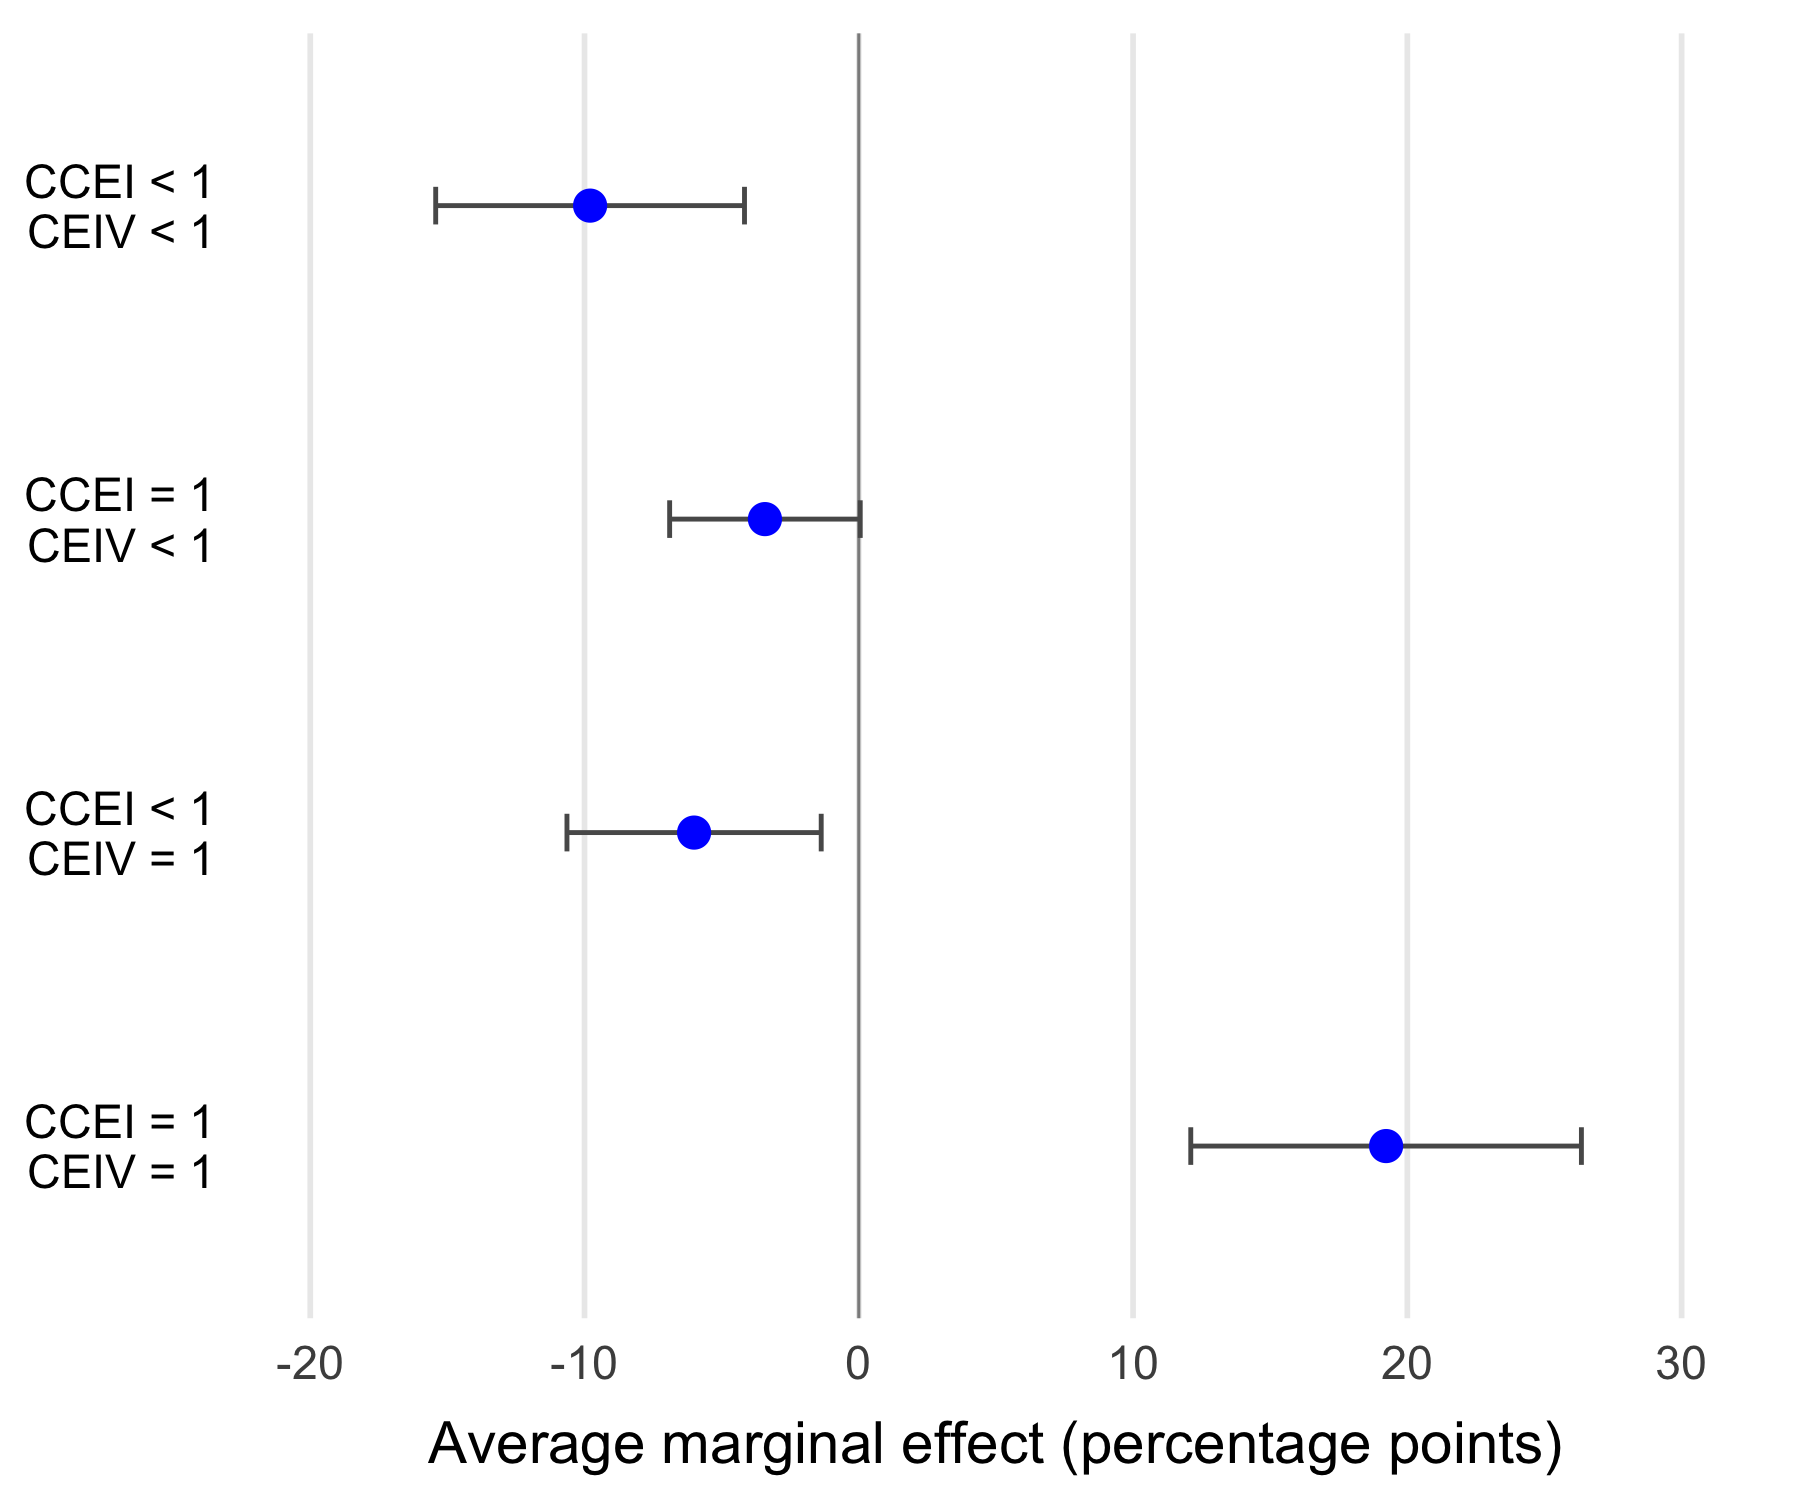
\includegraphics[width=\textwidth]{figure6_a_ame_maximum.png}
\caption{$\text{CCEI}_{\text{max},gt}$}\end{subfigure}\hfill
\begin{subfigure}[b]{0.485\textwidth}\centering
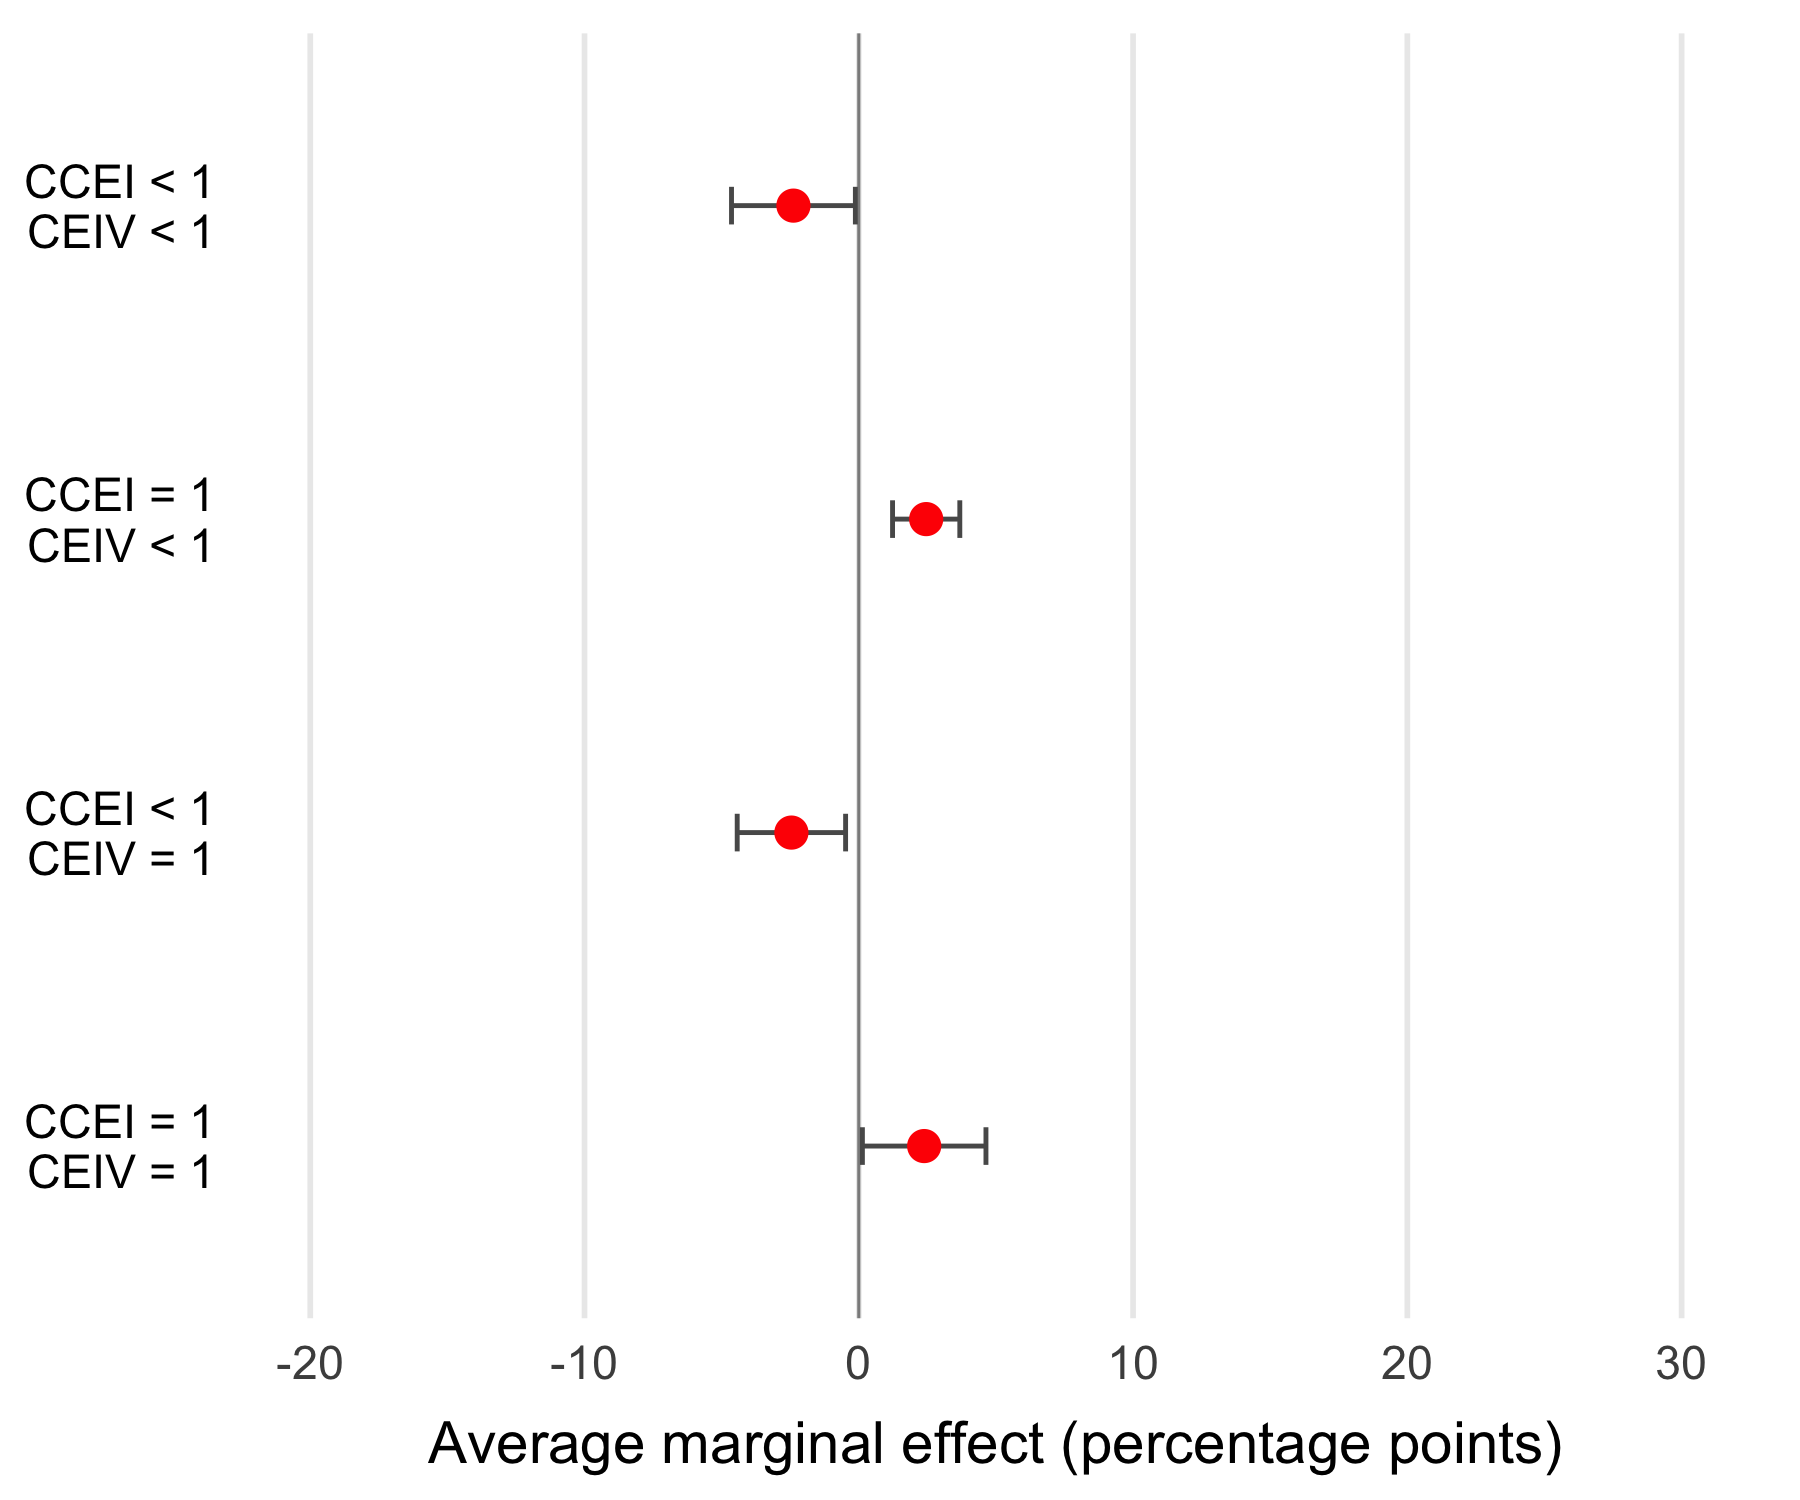
\includegraphics[width=\textwidth]{figure6_a_ame_minimum.png}
\caption{$\text{CCEI}_{\text{min},gt}$}\end{subfigure}
\end{figure}
\small
\textit{Notes:} Pooled multinomial-logit average marginal effects, expressed in
percentage points for a 0.1 increase in the indicated member's individual CCEI.
These are scaled average derivatives, not exact finite probability changes.
Both individual CCEIs enter jointly with Table 5 column (3)'s student, friendship,
and choice-pattern controls and class fixed effects. Risk-aversion controls are
excluded. All 1,304 pair-waves from 652 pairs are included; 95\% confidence intervals
use standard errors clustered by 64 classes. The colors, panel dimensions, axis
limits, point styling, and confidence-bar format follow the existing Figure 6.

\medskip
Category shares, from top to bottom: 31.83\%, 8.97\%, 23.01\%, and 36.20\%.
Classification uses the supplied indices and the draft's $10^{-9}$ tolerance.
\clearpage
\begin{center}\large\textbf{Figure 6 variant: CEIV and CEIC}\end{center}
\begin{figure}[ht]\centering
\begin{subfigure}[b]{0.485\textwidth}\centering
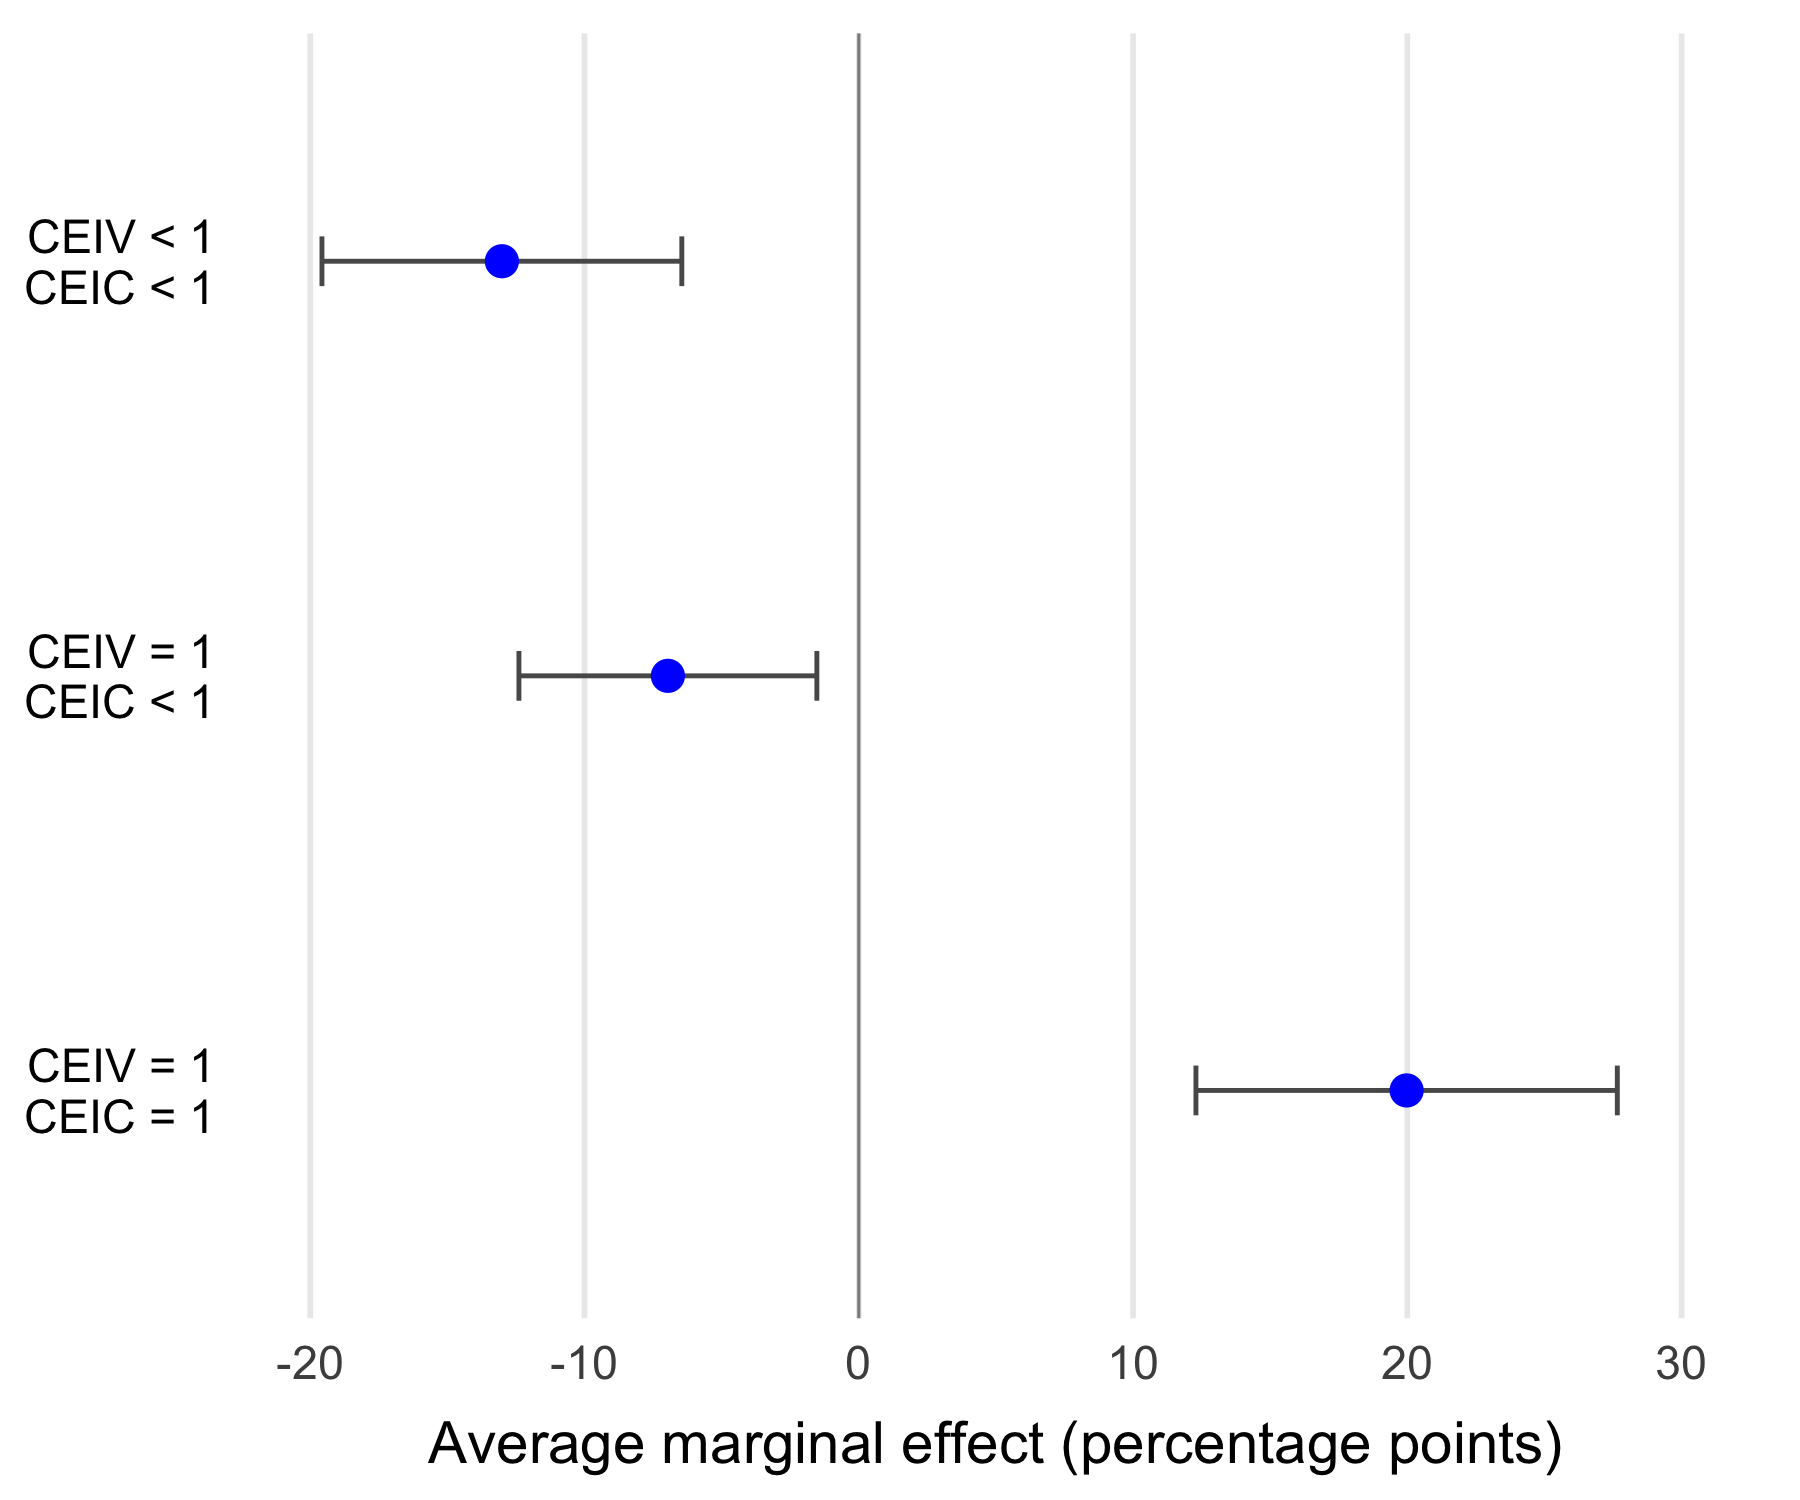
\includegraphics[width=\textwidth]{figure6_b_ame_maximum.png}
\caption{$\text{CCEI}_{\text{max},gt}$}\end{subfigure}\hfill
\begin{subfigure}[b]{0.485\textwidth}\centering
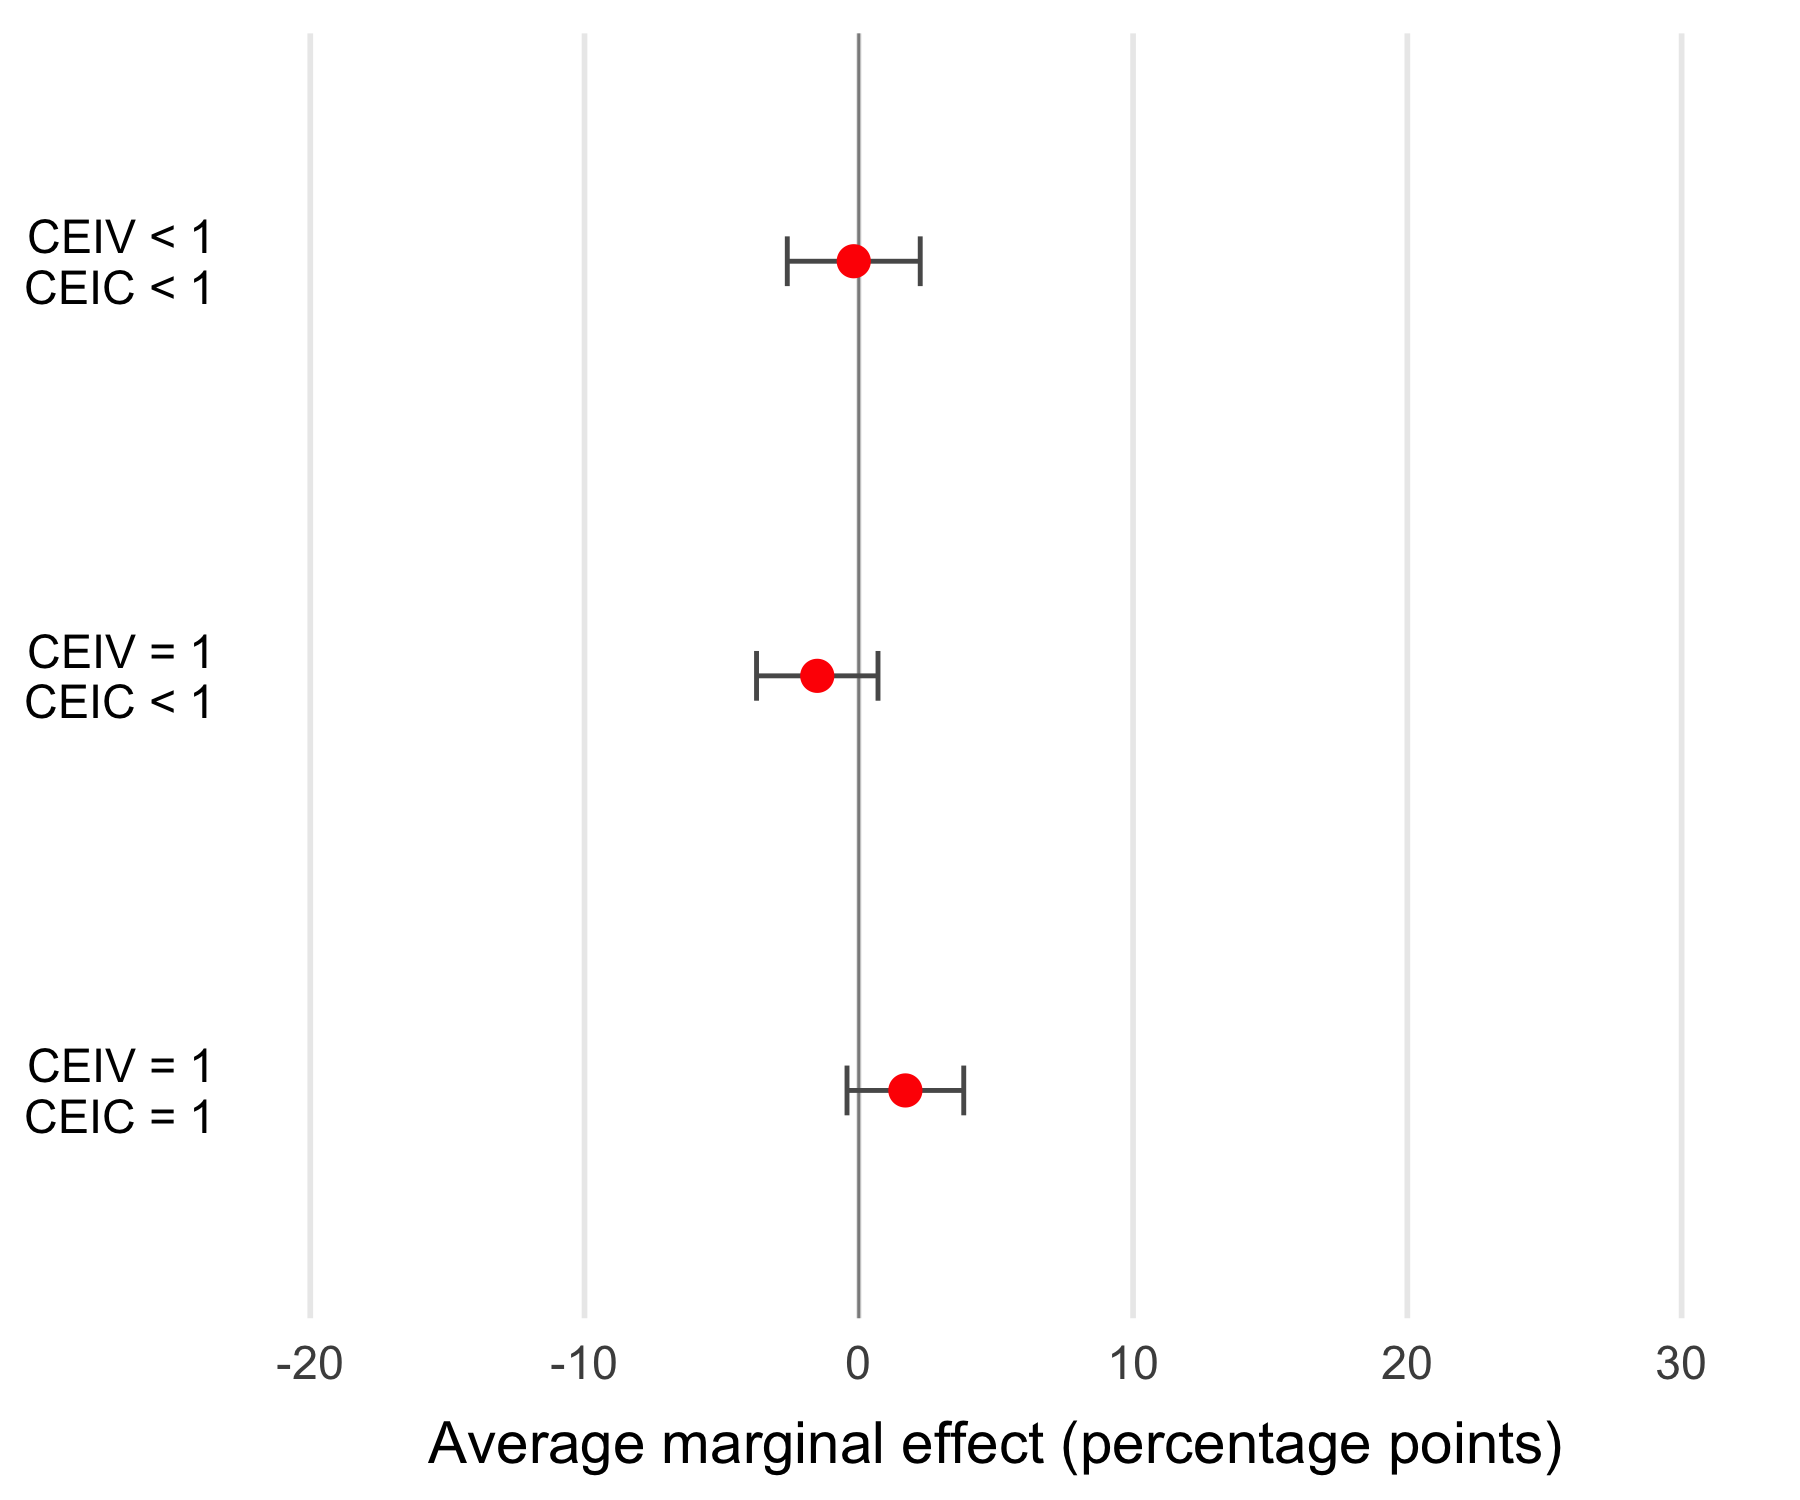
\includegraphics[width=\textwidth]{figure6_b_ame_minimum.png}
\caption{$\text{CCEI}_{\text{min},gt}$}\end{subfigure}
\end{figure}
\small
\textit{Notes:} Pooled multinomial-logit average marginal effects, expressed in
percentage points for a 0.1 increase in the indicated member's individual CCEI.
These are scaled average derivatives, not exact finite probability changes.
Both individual CCEIs enter jointly with Table 5 column (3)'s student, friendship,
and choice-pattern controls and class fixed effects. Risk-aversion controls are
excluded. All 1,304 pair-waves from 652 pairs are included; 95\% confidence intervals
use standard errors clustered by 64 classes. The colors, panel dimensions, axis
limits, point styling, and confidence-bar format follow the existing Figure 6.

\medskip
Category shares, from top to bottom: 40.80\%, 28.99\%, and 30.21\%.
Classification uses the supplied indices and the draft's $10^{-9}$ tolerance.

\medskip
There are no observations with CEIV below one and CEIC equal to one.
For 56 observations classified as CEIC below one, the reported numerical interval
has an upper bound of one; thus their classification may depend on finer numerical
resolution. They remain classified by their supplied point estimate. These rows
and the unresolved midpoint are identified in \texttt{precision\_audit.csv}.
\end{document}
